
\chapter{Investigation for truth 3-prong $\tauhad$ reconstructed as 2-prong}
\graphicspath{{2_Appendices/figures}}

\section*{Introduction}
    The reconstruction efficiency of the particle-level 3-prong $\tauhad$ decreases with increasing $\pt$ of the $\tauhad$, 
    particularly in the high-mass region of this analysis. When the 3-prong $\tauhad$ is not correctly reconstructed, 
    it is most often reconstructed as a 2-prong $\tauhad$, typically due to the failure to identify one of the charged pions. 
    For visible $\pt$ of the $\tauhad$ around 1 TeV, the probability of correctly reconstructing a 3-prong $\tauhad$ can be as low as 
    45\%~\cite{ATL-PHYS-PUB-2022-044}, as reported in Chapter~5. In such cases, the probability of it being 
    reconstructed as a 2-prong $\tauhad$ (3-to-2p migration) is approximately 30\%, while the probability of being 
    reconstructed as a 1-prong (3-to-1p migration) $\tauhad$ is around 15\%. The remaining probability is attributed 
    to reconstruction as a 4-prong (3-to-4 migration) or 0-prong (3-to-0 migration) $\tauhad$, both of which are negligible compared to other types of migration.

    From the perspective of this analysis, the 3-to-1p migration is not problematic, as reconstructed 
    1-prong $\tauhad$s are included in the signal region (SR). Likewise, the 3-to-4 and 3-to-0 migrations 
    are not concerning, as these rarely occur. By including reconstructed 2-prong $\tauhad$s in the SR, 
    the signal acceptance for the high-mass $G\rightarrow HH$ signal can potentially increase by 10\%. 
    However, the background composition must be carefully analysed to ensure that the inclusion of 
    2-prong $\tauhad$s does not significantly increase background contamination.

\section*{Event-selections}
    Table \ref{tab:n_evt_2p} shows the event yields in the $\mathrm{SR}_\mathrm{2p}$ and 
    $\mathrm{CR}_\mathrm{2p}$ regions. The selection on the charge of the muon and $\tauhad$ 
    is loosened to $q_{\mu}\times q_{\tauhad}\leq 0$, as the charge of the 2-prong 
    $\tauhad$ can only be 0 or $\pm 2$. The prongness selection is set to 2-prong, 
    ensuring that these regions are orthogonal to the SR and CR regions in the main analysis. 
    The TauID jet RNN score cut moves up from 0.05 to 0.15 to suppress the top background contamination.
    All other selection criteria for the $\mathrm{SR}_\mathrm{2p}$ and $\mathrm{CR}_\mathrm{2p}$ 
    regions remain identical to those used in the SR and CR regions of the main analysis.

    The same set of distributions as shown in the main text is presented in Figures~\ref{fig:2p_absDphi_bbtt} to \ref{fig:2p_qq}. 
    Good agreement between data and MC is observed across these distributions in $\mathrm{CR}_\mathrm{2p}$, 
    indicating that the 2-prong $\tauhad$ selection is also well-modelled in the MC simulation. 

    \begin{figure}[htbp]
        \centering
        \subfloat[]{
            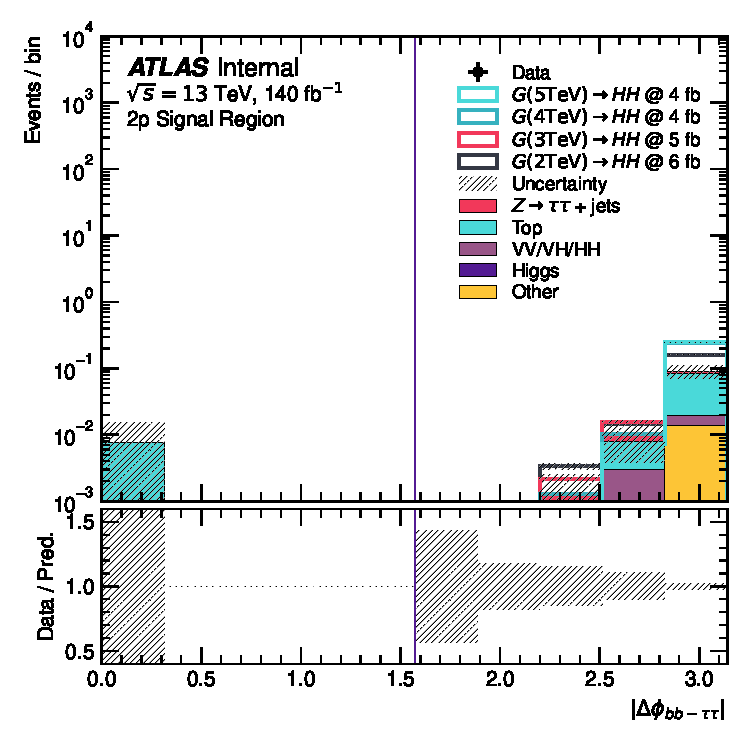
\includegraphics[width=0.50\textwidth]{abs_dPhi_bb_tt_SR.pdf}
            \label{fig:SR_2p_absDphi_bbtt}
        }
        %\hfill
        \subfloat[]{
            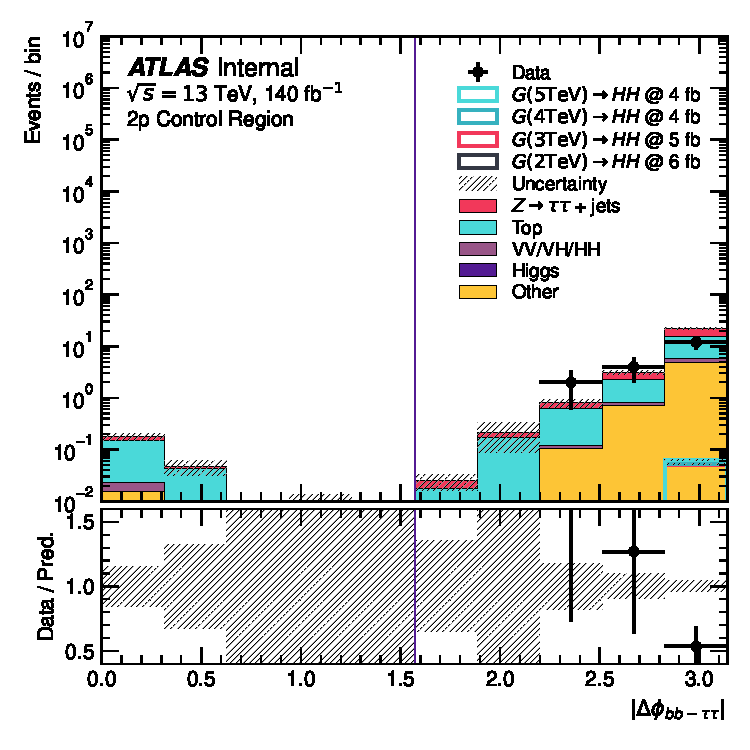
\includegraphics[width=0.50\textwidth]{abs_dPhi_bb_tt_CR.pdf}
            \label{fig:CR_2p_absDphi_bbtt}
        }
        \caption{
            The distribution of the $\absdPhibbtt$ in the SR (\protect\subref{fig:SR_2p_absDphi_bbtt}), and CR (\protect\subref{fig:CR_2p_absDphi_bbtt}).
        }    
        \label{fig:2p_absDphi_bbtt}
    \end{figure}

    \begin{figure}[htbp]
        \centering
        \subfloat[]{
            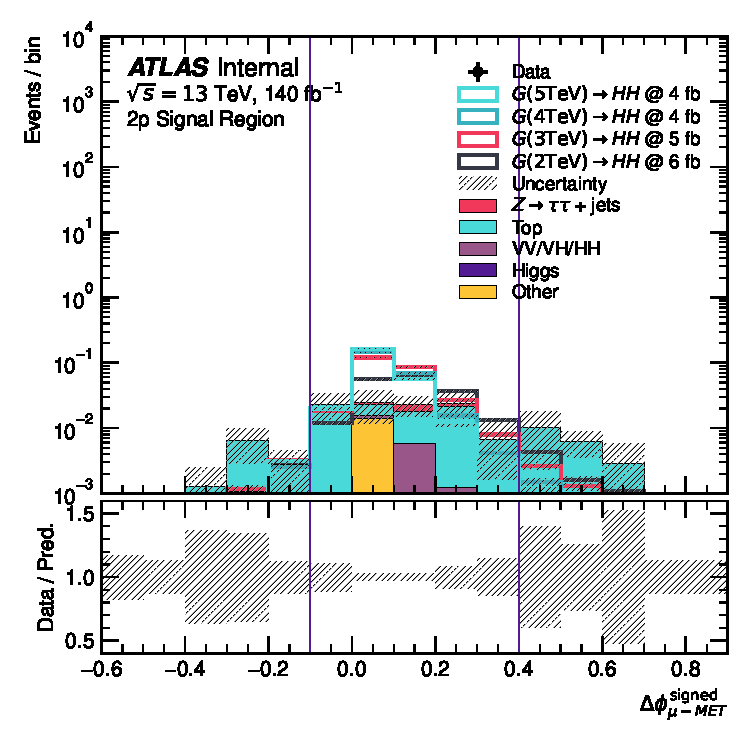
\includegraphics[width=0.50\textwidth]{dPhi_mu_met_SR.pdf}
            \label{fig:SR_2p_dPhi_mu_met}
        }
        %\hfill
        \subfloat[]{
            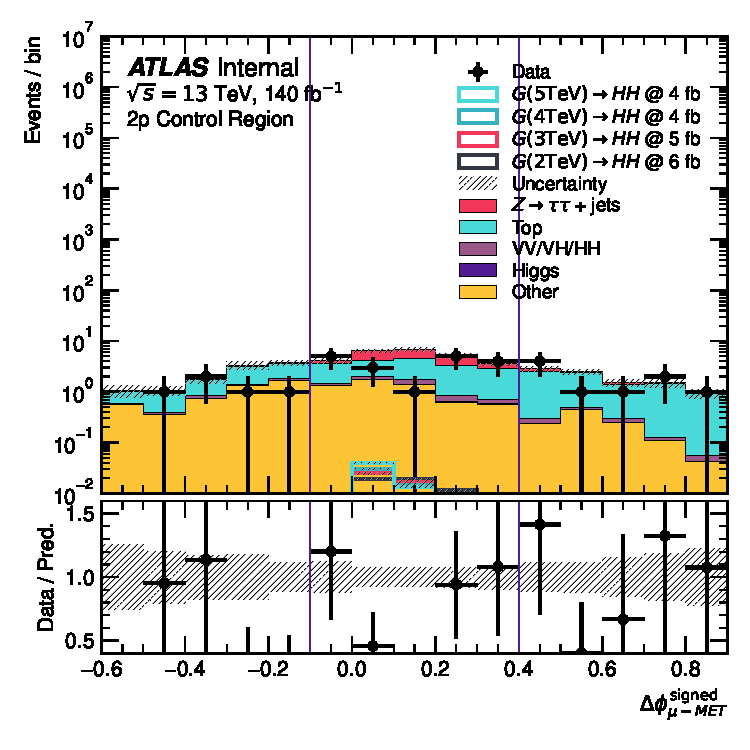
\includegraphics[width=0.50\textwidth]{dPhi_mu_met_CR.pdf}
            \label{fig:CR_2p_dPhi_mu_met}
        }
        \caption{
            The distribution of the $\dPhiMuMet$ in the SR (\protect\subref{fig:SR_2p_dPhi_mu_met}), and CR (\protect\subref{fig:CR_2p_dPhi_mu_met}).
        }
        \label{fig:2p_dPhi_mu_met}
    \end{figure}

    \begin{figure}[htbp]
        \centering
        \subfloat[]{
            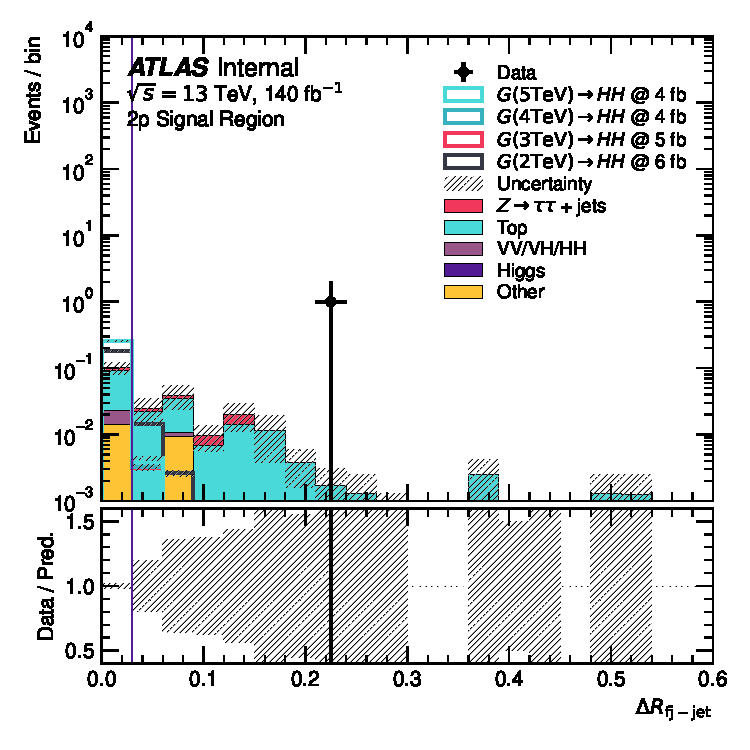
\includegraphics[width=0.50\textwidth]{dR_fj_jet_SR.pdf}
            \label{fig:SR_2p_dR_jfj}
        }
        %\hfill
        \subfloat[]{
            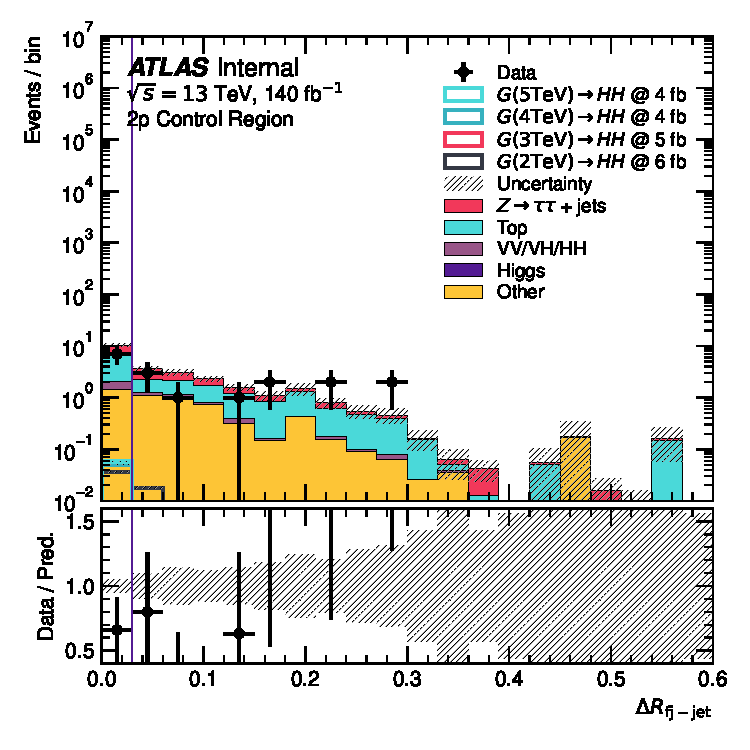
\includegraphics[width=0.50\textwidth]{dR_fj_jet_CR.pdf}
            \label{fig:CR_2p_dR_jfj}
        }
        \caption{
            The distribution of the $\dRjfj$ in the SR (\protect\subref{fig:SR_2p_dR_jfj}), and CR (\protect\subref{fig:CR_2p_dR_jfj}).
        }
        \label{fig:2p_dR_jfj}
    \end{figure}

    \begin{figure}[htbp]
        \centering
        \subfloat[]{
            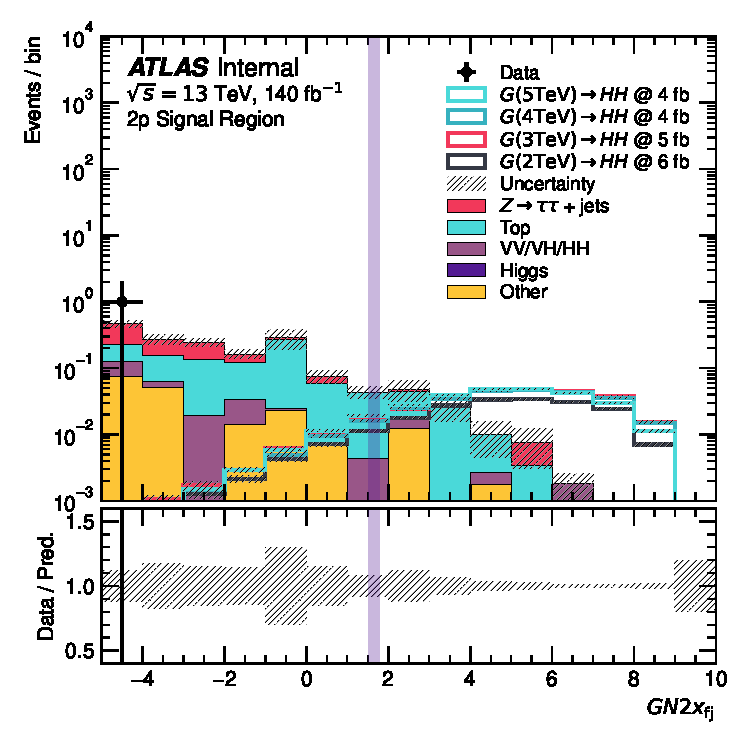
\includegraphics[width=0.50\textwidth]{fj_GN2x_SR.pdf}
            \label{fig:SR_2p_GN2bb}
        }
        %\hfill
        \subfloat[]{
            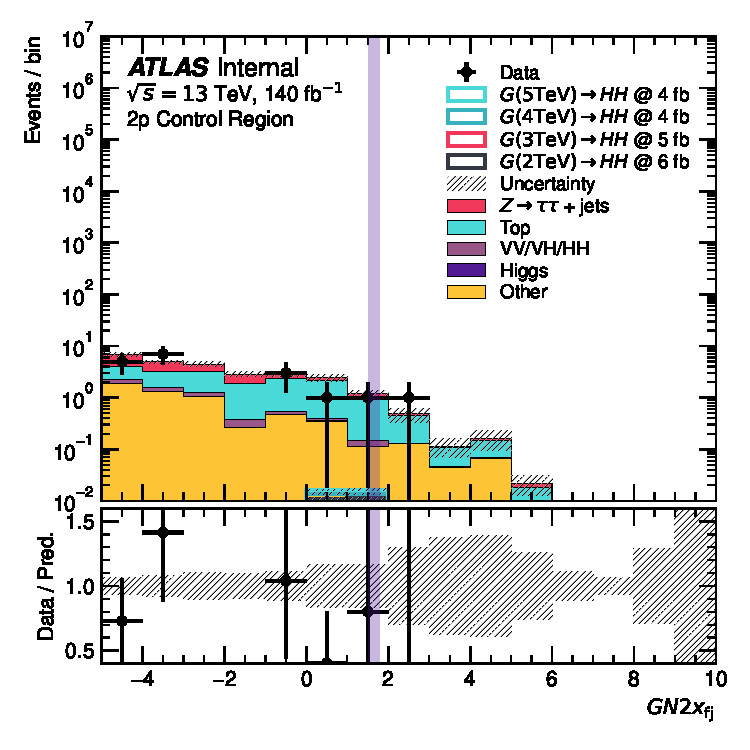
\includegraphics[width=0.50\textwidth]{fj_GN2x_CR.pdf}
            \label{fig:CR_2p_GN2bb}
        }
        \caption{
            The distribution of the $\GNTwoXFj$ in the SR (\protect\subref{fig:SR_2p_GN2bb}), and CR (\protect\subref{fig:CR_2p_GN2bb}). 
            The translucent band indicates the cut value of ``QCD1.55\%'' GN2x WP, ranging from 1.6 to 1.7 in the region where the fatjet mass is between 90 and 160 GeV.
        }
        \label{fig:2p_GN2bb}
    \end{figure}

    \begin{figure}[htbp]
        \centering
        \subfloat[]{
            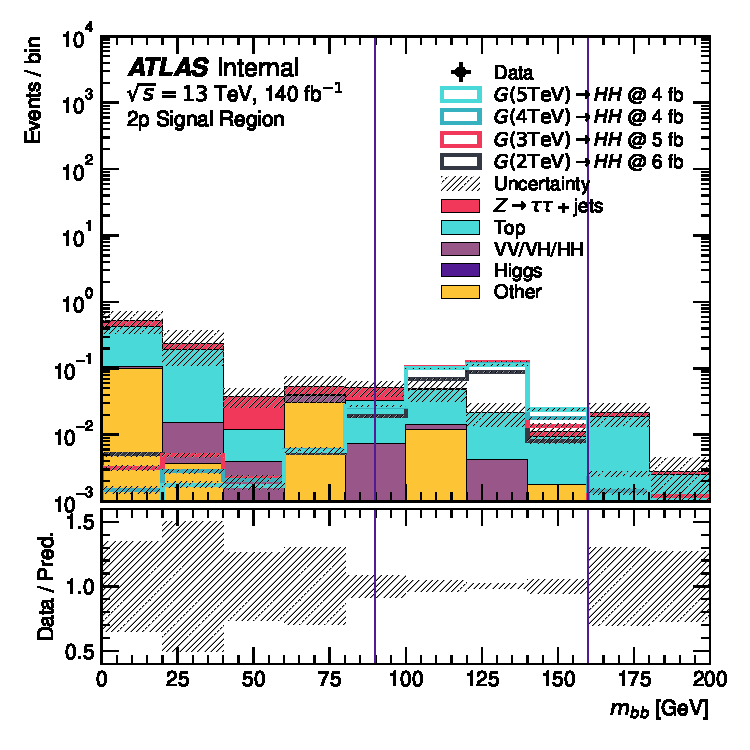
\includegraphics[width=0.50\textwidth]{M_bb_SR.pdf}
            \label{fig:SR_2p_mbb}
        }
        %\hfill
        \subfloat[]{
            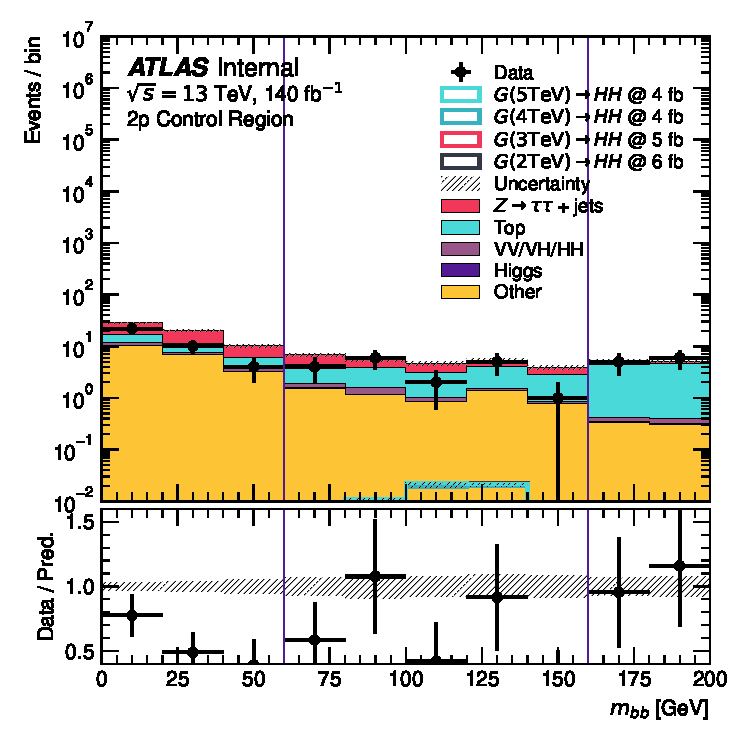
\includegraphics[width=0.50\textwidth]{M_bb_CR.pdf}
            \label{fig:CR_2p_mbb}
        }
        \caption{
            The distribution of the $\mbb$ in the SR (\protect\subref{fig:SR_2p_mbb}), and CR (\protect\subref{fig:CR_2p_mbb}).
        }
        \label{fig:2p_mbb}
    \end{figure}

    \begin{figure}[htbp]
        
        \centering
        \subfloat[]{
            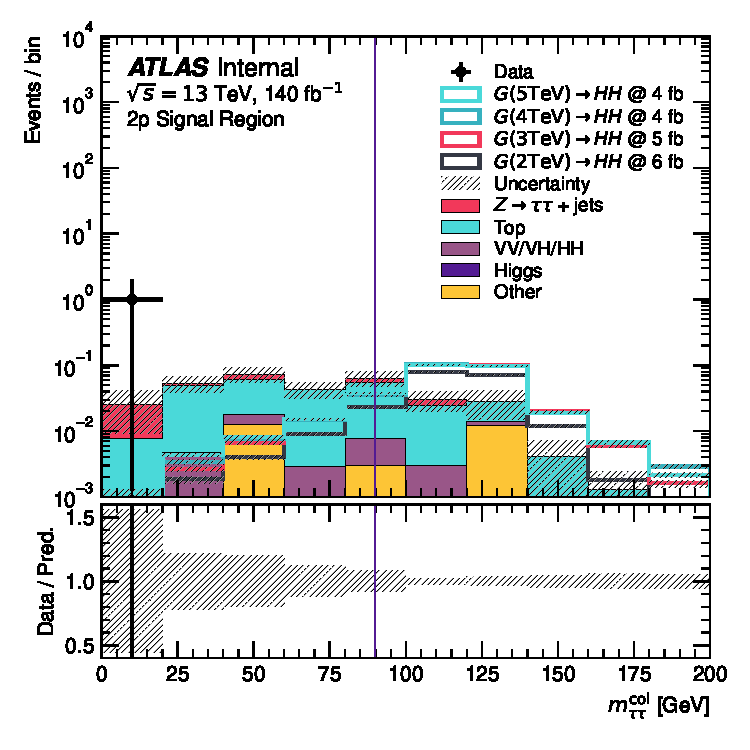
\includegraphics[width=0.50\textwidth]{M_tt_SR.pdf}
            \label{fig:SR_2p_mtt}
        }
        %\hfill
        \subfloat[]{
            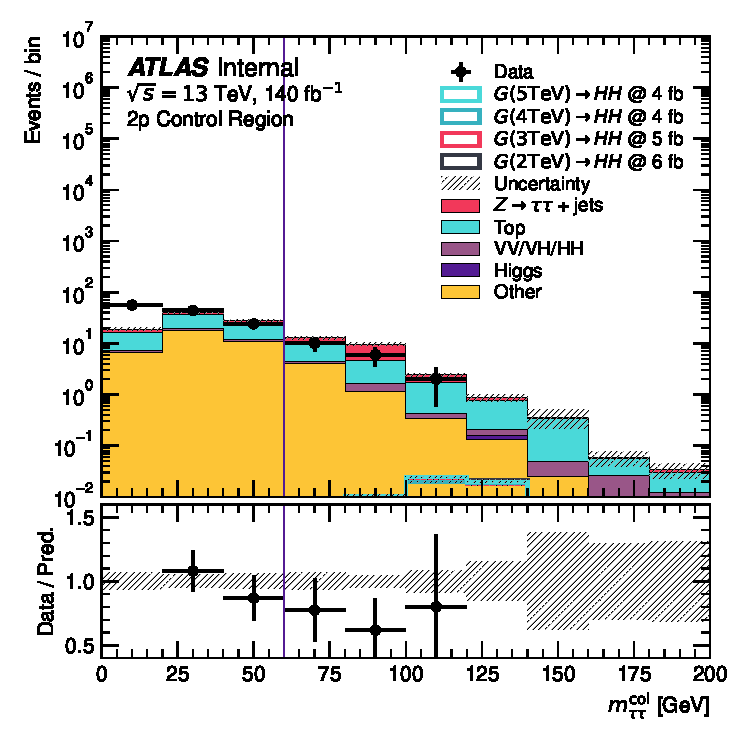
\includegraphics[width=0.50\textwidth]{M_tt_CR.pdf}
            \label{fig:CR_2p_mtt}
        }
        \caption{
            The distribution of the $\mttcol$ in the SR (\protect\subref{fig:SR_2p_mtt}), and CR (\protect\subref{fig:CR_2p_mtt}).
        }
        \label{fig:2p_mtt}
    \end{figure}   

    \begin{figure}[htbp]
        \centering
        \subfloat[]{
            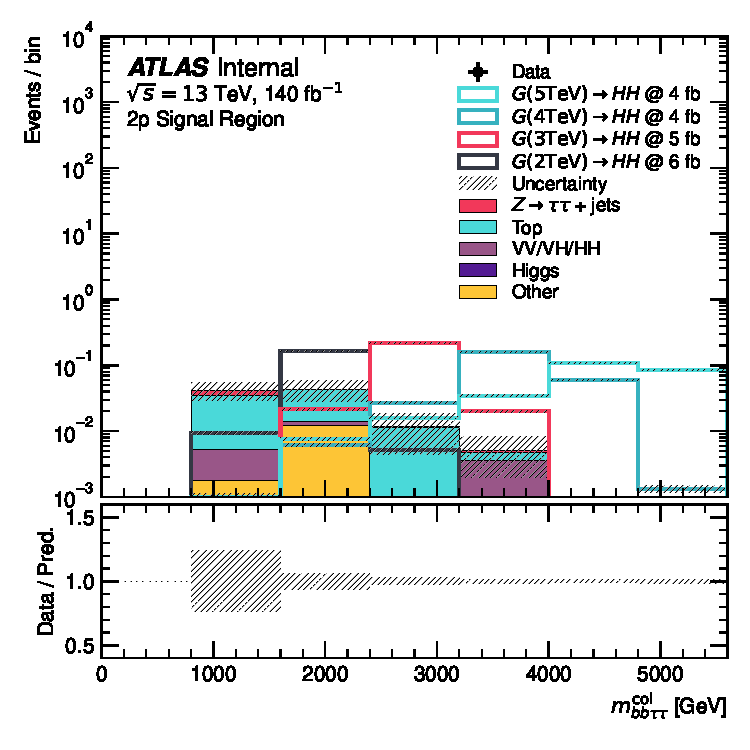
\includegraphics[width=0.50\textwidth]{M_bbtt_SR.pdf}
            \label{fig:SR_2p_mbbtt}
        }
        %\hfill
        \subfloat[]{
            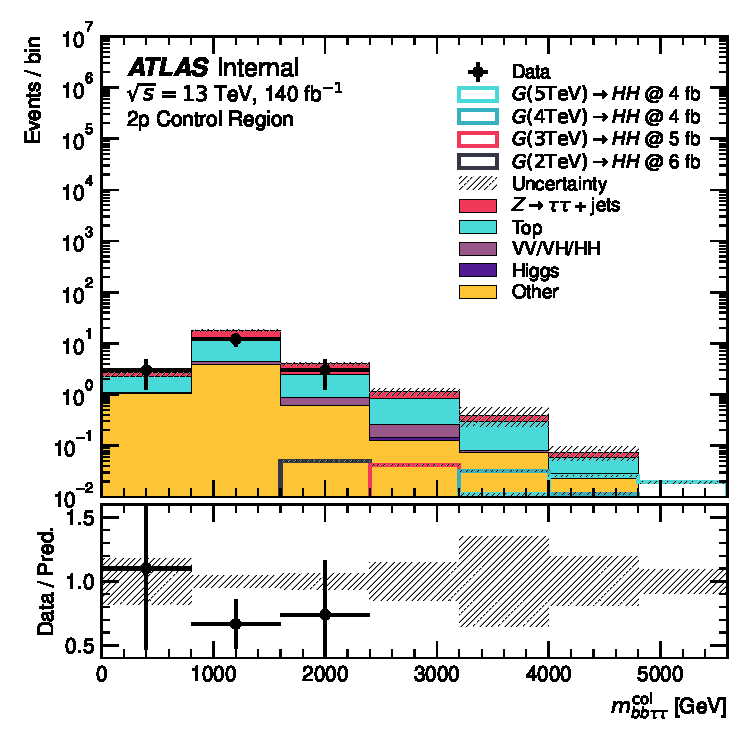
\includegraphics[width=0.50\textwidth]{M_bbtt_CR.pdf}
            \label{fig:CR_2p_mbbtt}
        }
        \caption{
            The distribution of the $\mbbttcol$ in the SR (\protect\subref{fig:SR_2p_mbbtt}), and CR (\protect\subref{fig:CR_2p_mbbtt}).
            The $\mbbttcol$ distribution extends to lower values in the CR than in the SR due to the relaxed $\mttcol$ and $\mbb$ requirements.  
            This is because lower values of $\mttcol$ and $\mbb$ in the CR allow di-$\tau$ and $b\bar{b}$ systems at 
            lower $\pt$ to be produced whilst still satisfying the condition $\Delta{R} < 0.4$.
        }
        \label{fig:2p_mbbtt}
    \end{figure}
    \begin{figure}[htbp]
        
        \centering
        \subfloat[]{
            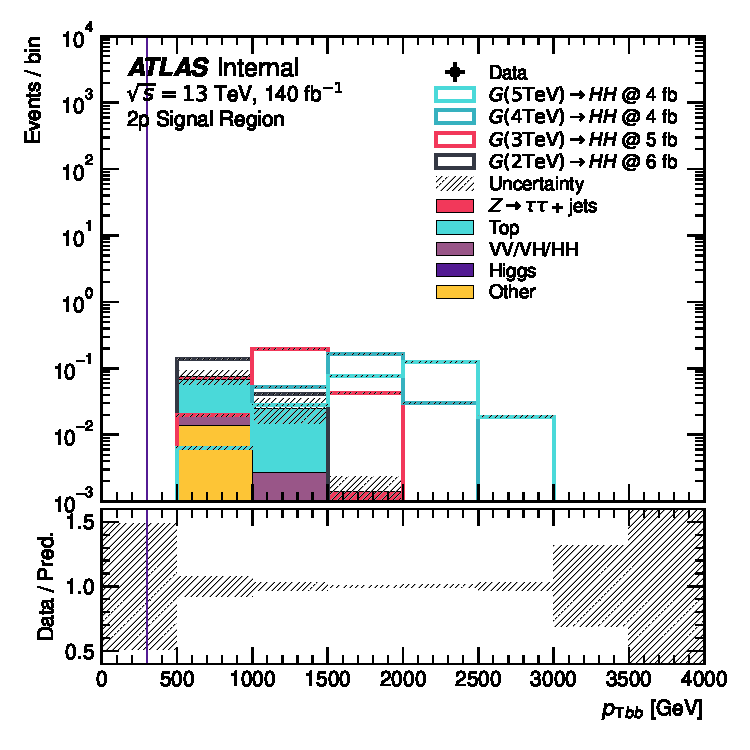
\includegraphics[width=0.50\textwidth]{pT_bb_SR.pdf}
            \label{fig:SR_2p_pTbb}
        }
        %\hfill
        \subfloat[]{
            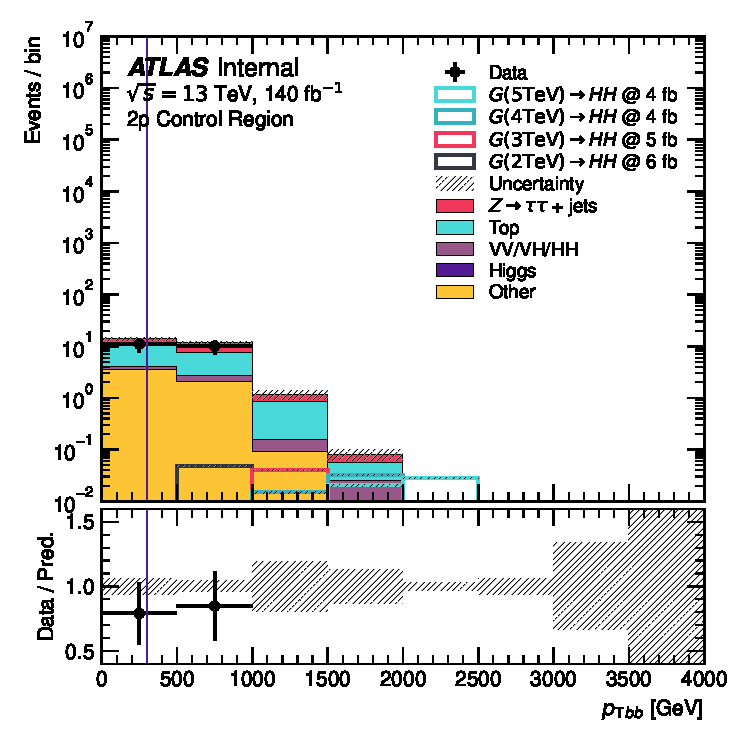
\includegraphics[width=0.50\textwidth]{pT_bb_CR.pdf}
            \label{fig:CR_2p_pTbb}
        }
        \caption{
            The distribution of the $\ptbb$ in the SR (\protect\subref{fig:SR_2p_pTbb}), and CR (\protect\subref{fig:CR_2p_pTbb}).
            The $\ptbb$ distribution extends to lower values in the CR than in the SR due to the relaxed $\mttcol$ and $\mbb$ requirements.  
            This is because lower values of $\mttcol$ and $\mbb$ in the CR allow di-$\tau$ and $b\bar{b}$ systems at 
            lower $\pt$ to be produced whilst still satisfying the condition $\Delta{R} < 0.4$.
        }
        \label{fig:2p_pTbb}
    \end{figure}

    \begin{figure}[htbp]
        
        \centering
        \subfloat[]{
            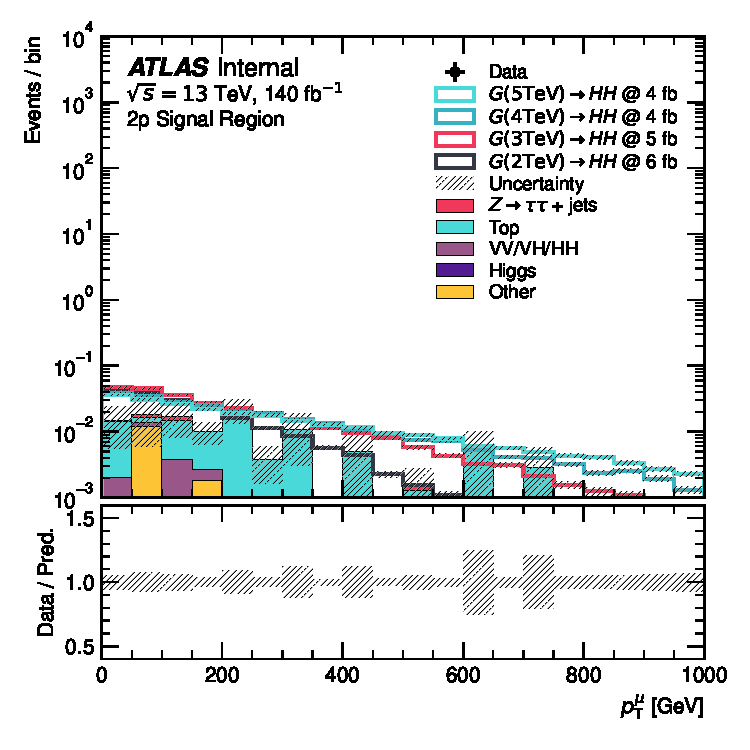
\includegraphics[width=0.50\textwidth]{pt_muon_SR.pdf}
            \label{fig:SR_2p_pTmu}
        }
        %\hfill
        \subfloat[]{
            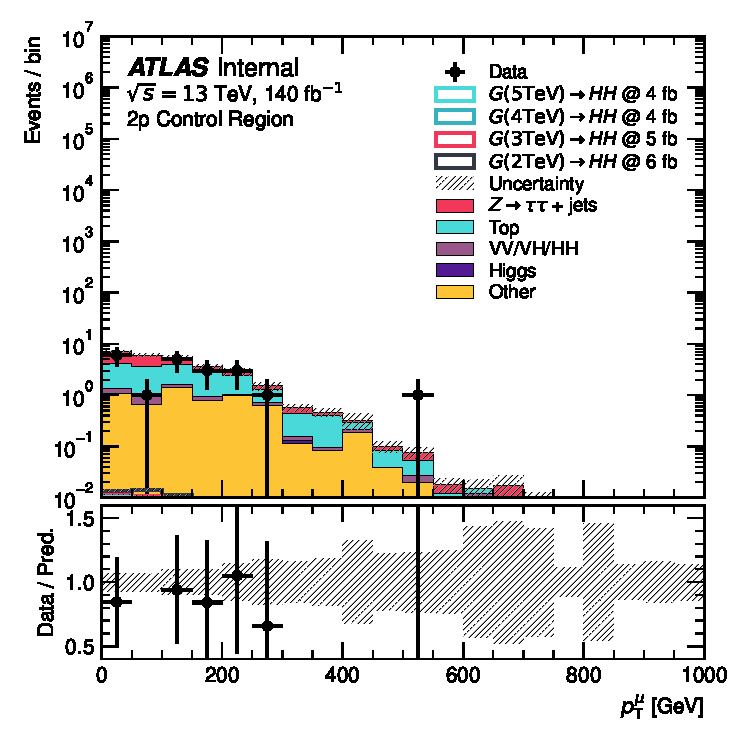
\includegraphics[width=0.50\textwidth]{pt_muon_CR.pdf}
            \label{fig:CR_2p_pTmu}
        }
        \caption{
            The distribution of the $\ptmuon$ in the SR (\protect\subref{fig:SR_2p_pTmu}), and CR (\protect\subref{fig:CR_2p_pTmu}).
        }
        \label{fig:2p_pTmu}
    \end{figure}

    \begin{figure}[htbp]
        
        \centering
        \subfloat[]{
            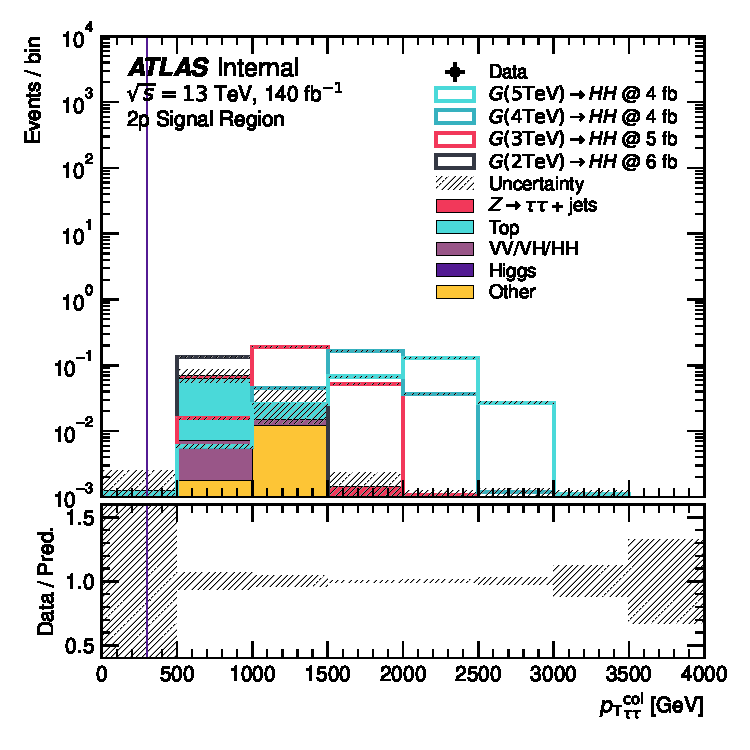
\includegraphics[width=0.50\textwidth]{pT_tt_SR.pdf}
            \label{fig:SR_2p_pTtt}
        }
        %\hfill
        \subfloat[]{
            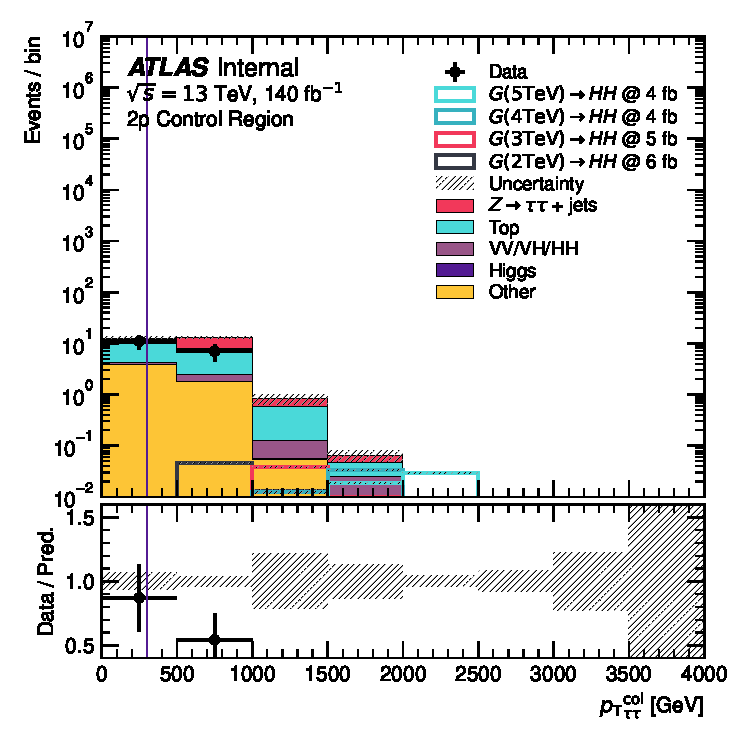
\includegraphics[width=0.50\textwidth]{pT_tt_CR.pdf}
            \label{fig:CR_2p_pTtt}
        }
        \caption{
            The distribution of the $\pttt$ in the SR (\protect\subref{fig:SR_2p_pTtt}), and CR (\protect\subref{fig:CR_2p_pTtt}).
            The $\pttt$ distribution extends to lower values in the CR than in the SR due to the relaxed $\mttcol$ and $\mbb$ requirements.  
            This is because lower values of $\mttcol$ and $\mbb$ in the CR allow di-$\tau$ and $b\bar{b}$ systems at 
            lower $\pt$ to be produced whilst still satisfying the condition $\Delta{R} < 0.4$.
        }
        \label{fig:2p_pTtt}
    \end{figure}

    \begin{figure}[htbp]
    
        \centering
        \subfloat[]{
            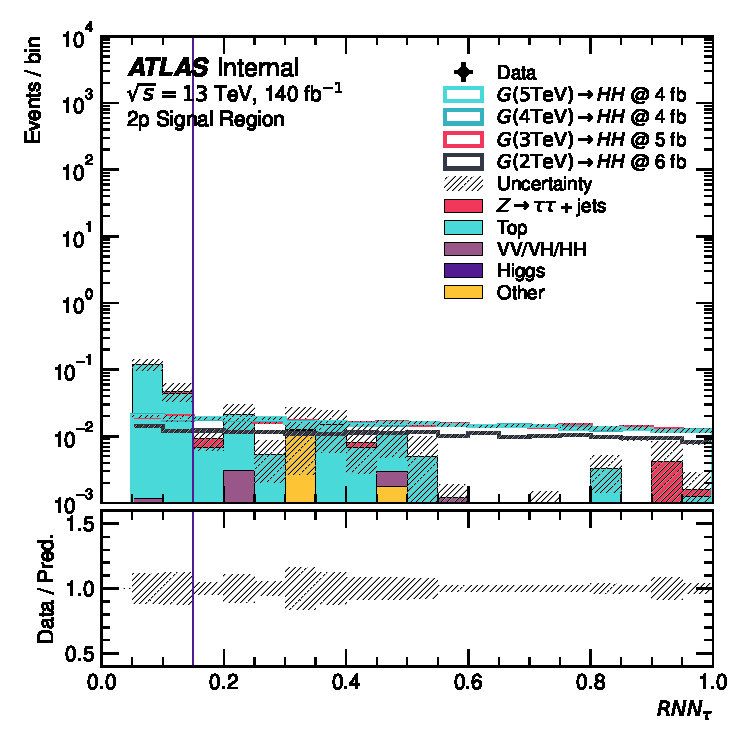
\includegraphics[width=0.50\textwidth]{tau_RNN_SR.pdf}
            \label{fig:SR_2p_tau_rnn}
        }
        %\hfill
        \subfloat[]{
            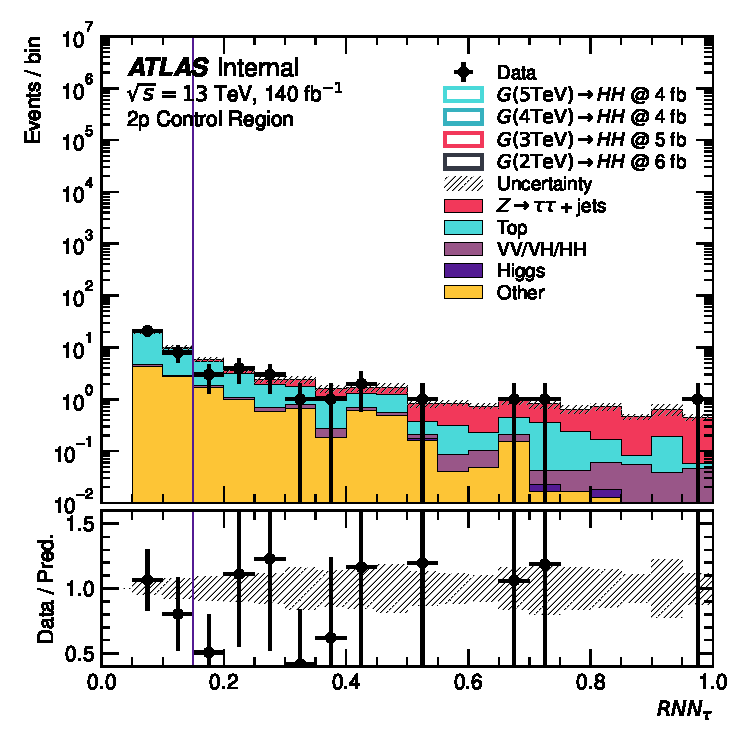
\includegraphics[width=0.50\textwidth]{tau_RNN_CR.pdf}
            \label{fig:CR_2p_tau_rnn}
        }
        \caption{
            The distribution of the $\rnn$ in the SR (\protect\subref{fig:SR_2p_tau_rnn}), and CR (\protect\subref{fig:CR_2p_tau_rnn}).
        }
        \label{fig:2p_tau_rnn}
    \end{figure}

    \begin{figure}[htbp]
        \centering
        \subfloat[]{
            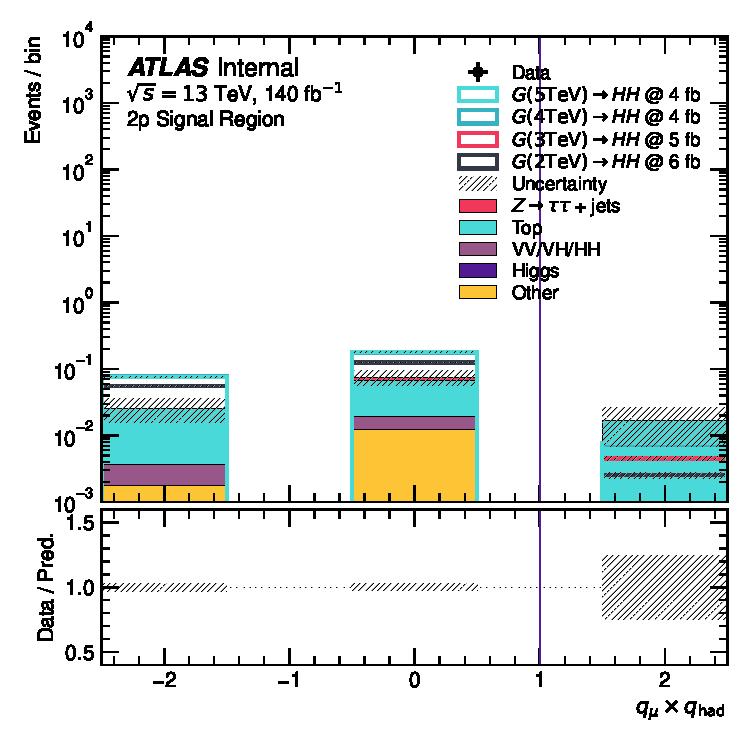
\includegraphics[width=0.50\textwidth]{qmu_qhad_SR.pdf}
            \label{fig:SR_2p_qq}
        }
        %\hfill
        \subfloat[]{
            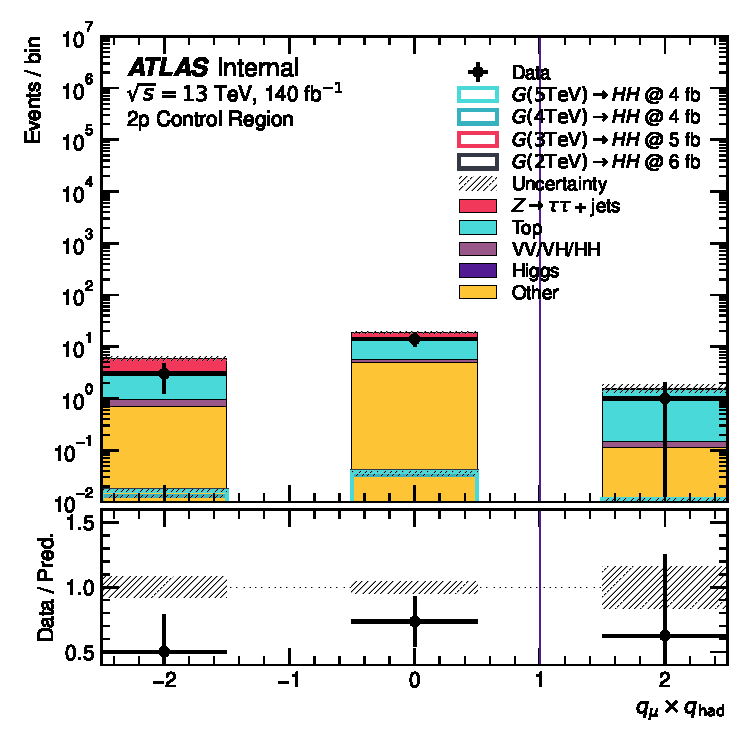
\includegraphics[width=0.50\textwidth]{qmu_qhad_CR.pdf}
            \label{fig:CR_2p_qq}
        }
        \caption{
            The distribution of the product of the $\tau\tau$ charges in the SR (\protect\subref{fig:SR_2p_qq}), and CR (\protect\subref{fig:CR_2p_qq}).
        }
        \label{fig:2p_qq}
    \end{figure}
    
    \begin{table}[htbp]
        \caption{Event yields in the SR 2p and CR 2p regions. 
        Apart from the different selection criteria for prongness and charge, the SR 2p and CR 2p regions are identical to the SR and CR regions in the main analysis.
        The uncertainties are statistical only. 
        The signal yields are shown with fixed cross-sections $\sigma(pp\rightarrow G\rightarrow HH) = 1$ fb.}
        \label{tab:n_evt_2p}
        \centering
        % \scriptsize
        \begin{tabular}{lrr}
            \toprule
                                                    & SR 2p                                   & CR 2p             \\
            \midrule
            Data                                    & 0                                       & $47 \pm 7$        \\
            SM MC total                             & $0.11$                                  & $46 \pm 3$        \\
            \midrule         
            jets + $Z\rightarrow\tau\tau$           & $0.01$                                  & $6.3  \pm 0.3$     \\
            diBoson                                 & $0.01$                                  & $1.5  \pm 0.1$     \\
            Top                                     & $0.10$                                  & $31   \pm 1$        \\
            Higgs                                   & $0.00$                                  & $0.03 \pm 0.02$   \\
            Others                                  & $0.01$                                  & $7    \pm 2$         \\
            \midrule         
            $G(2~\TeV)\rightarrow HH$               & $0.0343$                                & $0.0114 $         \\
            $G(3~\TeV)\rightarrow HH$               & $0.0598$                                & $0.0129 $         \\
            $G(4~\TeV)\rightarrow HH$               & $0.0725$                                & $0.0162 $         \\
            $G(5~\TeV)\rightarrow HH$               & $0.0731$                                & $0.0188 $         \\
            \bottomrule
        \end{tabular}
    \end{table}

\section*{Results}
    As expected, the signal efficiency in the $\mathrm{SR}_\mathrm{2p}$ is roughly 10\% of the signal efficiency in the main analysis for $G(3-5~\TeV)$. 
    The $\mathrm{SR}_\mathrm{2p}$ signal yield for $G(2~\TeV)$ is roughly 7\% of the signal yield in the SR, indicating 
    that the 3-to-2 migration is less prominent for the lower \pt \tauhad.
    The SM MC predicted 0.11 events in the $\mathrm{SR}_\mathrm{2p}$, the composition of which is different from the nominal SR, 
    with the $\ttbar$ being the dominant background. 
    Other major backgrounds appeared in the nominal SR, such as $Z\rightarrow\tau\tau$ and diBoson,
    are sources of genuine $\tmth$, which are suppressed by the 2-prong $\tauhad$ selection in the $\mathrm{SR}_\mathrm{2p}$. 
    In the $\mathrm{CR}_\mathrm{2p}$, genuine $\tmth$ backgrounds are also suppressed for the same reason, the $\ttbar$ contribution is promoted 
    to be the dominant background. 
\section*{Discussion}
    In exchange of the 10\% signal acceptance increase, 
    the $\mathrm{SR}_\mathrm{2p}$ region see a 10\% increase in the background contamination.
    We required a slightly tighter $\tauhad$ jet RNN score cut, which has the effect that 
    the background contamination is reduced
    significantly, without sacrificing much signal acceptance.
    Given that the SR and $\mathrm{SR}_\mathrm{2p}$ regions are essentially background-free, 
    and the fact that this analysis is heavily bottle-necked by the signal yield,
    the increase in the background contamination is acceptable.

    This analysis is the first in ATLAS to use the 2-prong $\tauhad$ in the signal region.
    With the 10\% increase in signal acceptance, the sensitivity of this analysis is expected improve roughly linearly with the increase in signal acceptance.
    The expected upper-limits, incorporating the $\mathrm{SR}_\mathrm{2p}$ contributions, are shown in Table~\ref{tab:limits_w_2p}.
    The Brazil band plots are shown in Figure~\ref{fig:limits_w_2p}.
    The limits are obtained with a 10-bin counting experiment, with the 2-prong analysis 
    concatenated to the main analysis. 
    \begin{table}[htbp]
        \caption{
            The expected and observed 95\% CL limits on the $\sigma(G\rightarrow HH)$ on various mass points. 
            Limits are obtained with the 2-prong analysis concatenated to the main analysis.
        }
        \label{tab:limits_w_2p}
        \centering
        % \scriptsize
        \begin{tabular}{lrrrrrr}
            \toprule
            Mass [GeV]   & $-2\sigma$ [fb]   & $-1\sigma$ [fb]   & Exp. [fb]   & $+1\sigma$ [fb]   & $+2\sigma$ [fb] & Observed [fb]\\
            \midrule
            2000         & 4.3               & 5.1               & 5.7         & 8.0               & 11.9            & 5.4\\
            3000         & 2.9               & 3.5               & 4.1         & 4.7               & 6.5             & 3.8\\
            4000         & 3.1               & 3.2               & 3.6         & 4.1               & 5.3             & 3.5\\
            5000         & 2.9               & 3.4               & 3.8         & 4.3               & 5.4             & 3.8\\
            \bottomrule
        \end{tabular}
    \end{table}
    \begin{figure}[htbp]
        \centering
        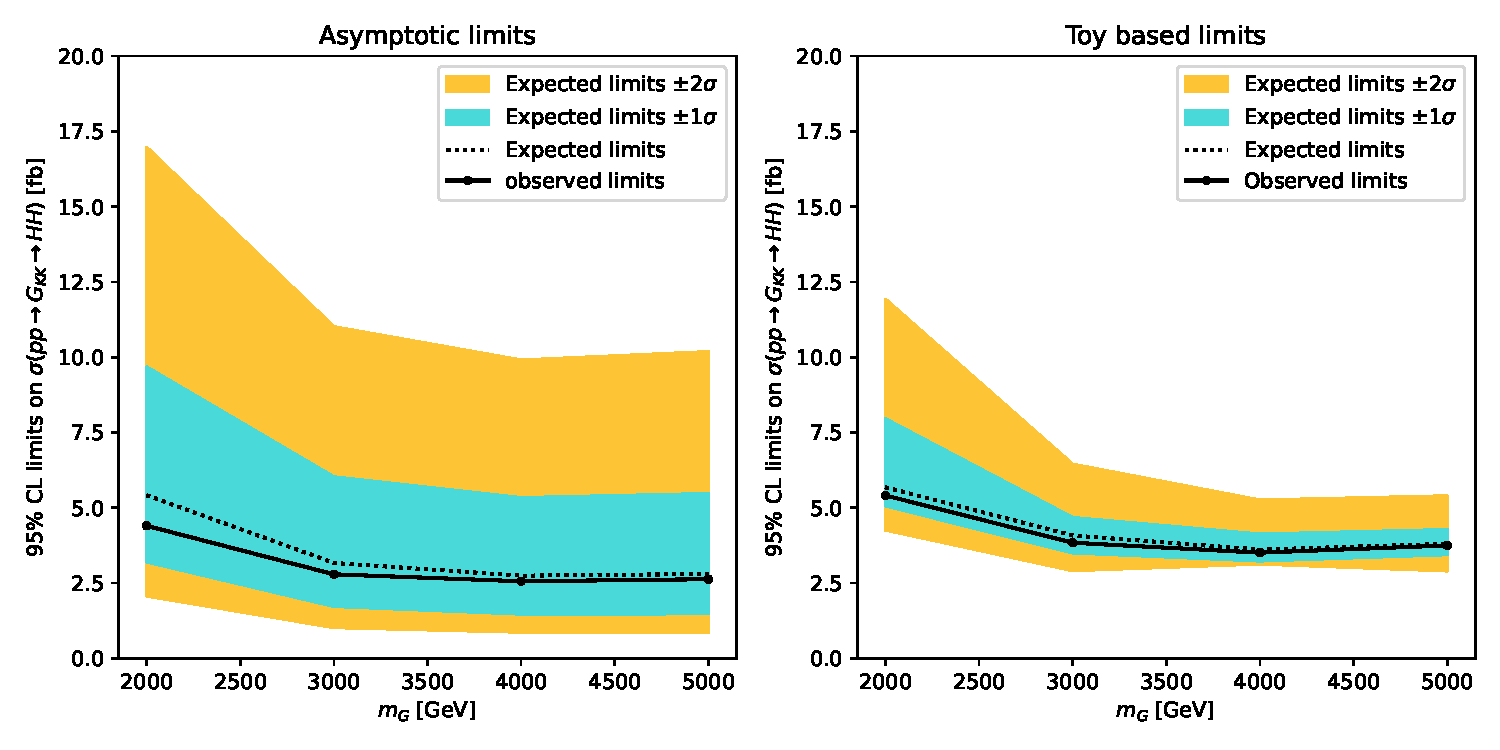
\includegraphics[width=1.0\textwidth]{limits_all_w_2p.pdf}
        \caption{
            The expected and observed 95\% CL limits on the $\sigma(G\rightarrow HH)$ on various mass points. 
            Limits are obtained with the 2-prong analysis concatenated to the main analysis.
        }
        \label{fig:limits_w_2p}
    \end{figure}